\chapter{Nevek és listák}
\thispagestyle{empty}

\section{Cellák elnevezése }

Cellákhoz és cellatartományokhoz neveket rendelhetünk. Az
elnevezett cellákra és cellatartományokra képletekben a
nevükkel hivatkozhatunk. Ez megkönnyíti a képletek
értelmezését és másolását. Neveket tartalmazó
képleteket másolva, azok nem változnak. Érdemes olyan
tartományhoz vagy cellához nevet rendelni, amelyeket abszolút
hivatkozásként használunk a képletekben.

Neveket legegyszerűbben úgy hozhatunk létre, hogy a
szükséges cella vagy cellatartomány kijelölése után a
névdobozba kattintunk egérrel, kitöröljük az ott lévő
cellahivatkozást és beírjuk a nevet (\ref{CellákElnevezése} ábra).

\begin{figure}[!h]
\begin{center}
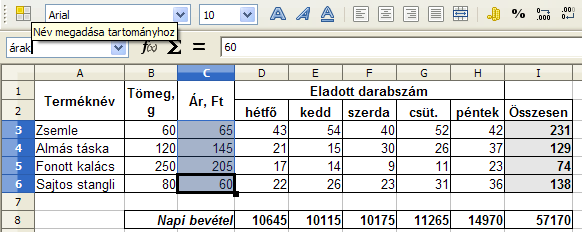
\includegraphics[width=14.395cm]{oocalcv2-img104.png}
\caption{Cellák elnevezése}\label{CellákElnevezése}
\end{center}
\end{figure}

\Aref{CellákElnevezése} ábrán a C3:C6 tartománynak az
,,árak'' nevet adtuk.

A Calcban használt nevek betűket és számokat tartalmazhatnak,
a speciális karakterek közül csak az aláhúzásjelet ( \_ )
és pontot ( . ). A név nem lehet lehetséges hivatkozásnév
sem.

A neveket létrehozhatunk a \textbf{Beszúrás} menüpont
\textbf{Nevek} --  \textbf{Meghatározás} paranccsal, vagy a Ctrl+F3
billentyűkombinációval (\ref{NevekMegadása} ábra). Az ablakban
módosíthatjuk a nevekhez tartozó cellahivatkozásokat és
törölhetjük is őket.

\begin{figure}[!h]
\begin{center}
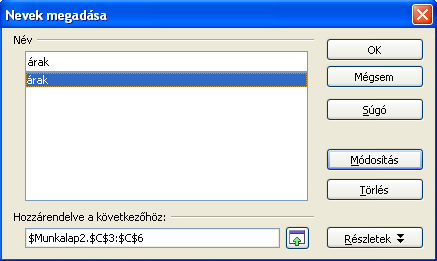
\includegraphics[width=11.562cm]{oocalcv2-img105.png}
\caption{Nevek megadása}\label{NevekMegadása}
\end{center}
\end{figure}


\section{23. feladat }

{\itshape
A negyedik feladatban kiszámított napi bevételt számítsuk ki
függvény és cellák elnevezése segítségével.}

A negyedik feladatban alkalmazott képlet
{\sffamily\bfseries{(=\$C\$3*D3+\$C\$4*D4+\$C\$5*D5+\$C\$6*D6)}}
szorzatok összege, amire találunk függvényt is a Calcban. Ez a
SZORZATÖSSZEG függvény.

A \textbf{SZORZATÖSSZEG} függvény
összeszorozza az adott tömbök megfelelő elemeit, és
eredményül a szorzatok összegét adja. Szintaxisa:
SZORZATÖSSZEG(tömb1; tömb2...tömb30).

Az előző képletet helyettesíthetjük a következő függvénnyel:\\
{\sffamily\bfseries{=SZORZATÖSSZEG(\$C\$3:\$C\$6;D3:D6)}}.
Mivel a C3:C6 tartománynak az ,,árak'' nevet adtuk:
{\sffamily\bfseries{=SZORZATÖSSZEG(árak;D3:D6)}} (\ref{23-feladatSUMPRODUCT} ábra).

\begin{figure}[!h]
\begin{center}
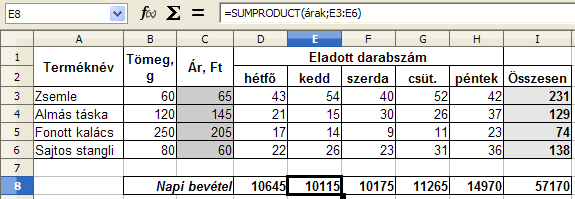
\includegraphics[width=15.212cm]{oocalcv2-img106.png}
\caption{23. feladat --  SZORZATÖSSZEG függvény}\label{23-feladatSUMPRODUCT}
\end{center}
\end{figure}


\section{Rendezett listák }

Cella másolásakor annak tartalmától függően a Calc
vagy másolást végez, vagy sorozattal tölti fel a cellákat.
Szöveges tartalom esetén általában megismétli a cella
tartalmát. Ez alól két kivétel van. Az egyik, ha a cellában a
szöveg után szám található. Ilyenkor másoláskor folytatja
a számozást. \Aref{CellákMásolása} ábrán látható három oszlop ezzel a
módszerrel lett létrehozva.

\begin{figure}[!h]
\begin{center}
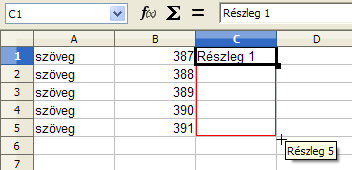
\includegraphics[width=8.312cm]{oocalcv2-img107.png}
\caption{Cellák tartalmának másolása}\label{CellákMásolása}
\end{center}
\end{figure}

Másolásnál a Ctrl billentyűt lenyomva tartva kikapcsolhatjuk a
számsorozat létrehozását.

A második kivétel, ha olyan szöveget írunk be, ami eleme a Calc
rendezett listáinak. Ezek a listák megtekinthetők az
\textbf{Eszközök} menüpont \textbf{Beállítások}
párbeszédablakban, az \textbf{OpenOffice.org Calc} --
\textbf{Rendezett listák} lehetőséget választva (\ref{RendezettListák}
ábra).

\begin{figure}[!h]
\begin{center}
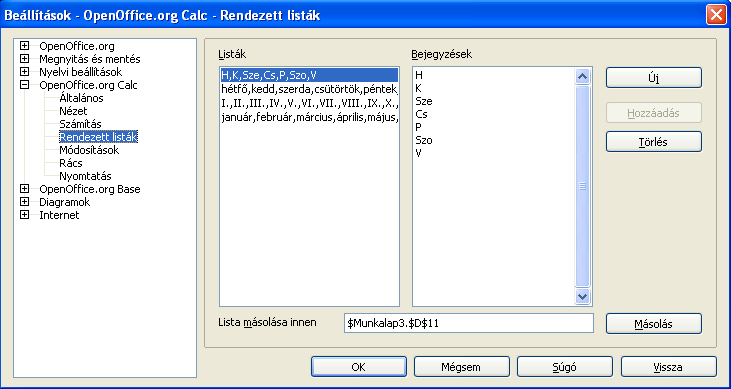
\includegraphics[width=14.999cm]{oocalcv2-img108.png}
\caption{Rendezett listák}\label{RendezettListák}
\end{center}
\end{figure}

Lehetőség van saját listák létrehozására is. Ehhez csak
be kell írni a listát egy tetszőleges tartományba és \aref{RendezettListák}
ábrán látható \textbf{Másolás} majd az \textbf{OK} gombra
kattintani. 


\section{Sorozatok létrehozása}

A Calcban egyszerűen létrehozhatunk növekvő számtani és
mértani sorozatokat. Írjuk be egy cellába a sorozat első
tagját, és jelöljük ki azt a tartományt, ahová a számsort
létre akarjuk hozni. Válasszuk a \textbf{Szerkesztés --
Kitöltés --  Sorozat} parancsot. 

\begin{figure}[!h]
\begin{center}
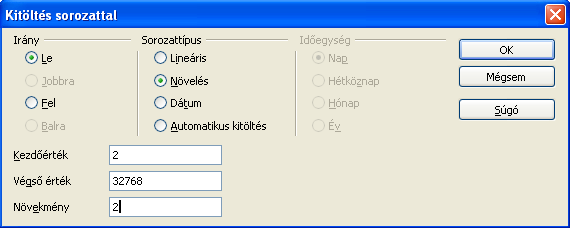
\includegraphics[width=12.081cm]{oocalcv2-img109.png}
\caption{Kitöltés sorozattal}\label{KitöltésSorozattal}
\end{center}
\end{figure}

\Aref{KitöltésSorozattal} ábrán látható beállításokkal mértani sorozat
jön létre, a sorozat hányadosa 2-vel egyenlő. Számtani
sorozatnál a sorozat különbségét kell a Növekmény mezőbe írni.

Dátumsorozatot is létrehozhatunk, a növekmény megadásán
kívül ilyenkor időegységet is választhatunk.


\section{Cellatartomány érvényesítése}

Az \textbf{Adatok} menüpont \textbf{Érvényesség}
párbeszédablakában beállíthatjuk, hogy egy cellába ne
beírással, hanem listából való kiválasztással
kerüljön adat. A lista egy sorból vagy oszlopból állhat, és
egyszerűbb, ha névvel azonosítjuk. Az \textbf{Engedélyezés}
résznél válaszuk a \textbf{Cellatartomány}t és a
\textbf{Forrás}hoz írjuk be a meghatározott nevet.


\section{24. feladat}

{\itshape
Módosítsuk a 20. feladatot, hogy az A19 cellában választható
legyen bármelyik kód az A2:A17 cellatartományból.}

Első lépésként jelöljük ki az A2:A17 cellatartományt
és adjuk neki a \textbf{kódok} nevet. Az A19 cellát választva
az \textbf{Érvényesség} párbeszédablakban válasszuk a
\textbf{Cellatartomány}t és a forráshoz írjuk a
 \textbf{kódok} nevet. Ezután az A19 cellára kattintva a cella
jobb oldalán egy nyilat ábrázoló gomb jelenik meg, arra
kattintva megjelenik a lista (\ref{24-feladat} ábra).

\begin{figure}[!h]
\begin{center}
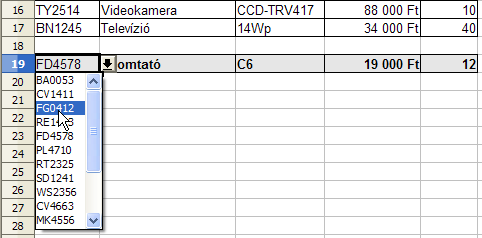
\includegraphics[width=12.751cm]{oocalcv2-img110.png}
\caption{24. feladat}\label{24-feladat}
\end{center}
\end{figure}

Egérrel választhatunk a listából és a cella azt az értéket
veszi fel. A B19:E19 tartományban az FKERES függvény megkeresi az
adott kódhoz tartozó adatokat.

